\documentclass{article}

% Language setting
% Replace `english' with e.g. `spanish' to change the document language
\usepackage[english]{babel}

% Set page size and margins
% Replaced `letterpaper' with `a4paper' for UK/EU standard size
\usepackage[a4paper,top=2cm,bottom=2cm,left=3cm,right=3cm,marginparwidth=1.75cm]{geometry}

% Useful packages
\usepackage{amsmath}
\usepackage{graphicx}
\usepackage{float}

\usepackage{natbib}
\bibliographystyle{apalike}
%\bibliographystyle{abbrv}
\usepackage[english]{babel}
\usepackage{booktabs} % Allows the use of \toprule, \midrule and \bottomrule in tables
\usepackage{subcaption}
\usepackage{xcolor}
\usepackage{tcolorbox}
\usepackage{tabularx}
\usepackage{textcomp}
\usepackage{comment}
\usepackage{mhchem}
\usepackage{fixltx2e}
\usepackage{MnSymbol,wasysym}
%\captionsetup[figure]{labelformat=empty}
\usepackage{hyperref}
\usepackage{verbatim}
\usepackage[parfill]{parskip}
%\usepackage[none]{hyphenat}

\hypersetup{
colorlinks=true,
citecolor=violet,
linkcolor=purple,   
urlcolor=blue}

\title{Tables, Images, Formulas and Citations}
\author{Anthea Alberto \& Overleaf}
\date{} % do not print the date

\begin{document}
\maketitle

\begin{abstract}
\noindent This is a document that will give you examples of some of the topics covered in the \LaTeX{} course organised by GRACE at the University of Basel. You can also find this document plus its source code on the course's \href{https://github.com/RISE-UNIBAS/grace_latex}{GitHub repo}.
\end{abstract}

\section{Introduction}

This document is based on a sample provided by Overleaf that aims to explain some of the core functionalities of \LaTeX{}. You can find the original \href{https://www.overleaf.com/latex/templates/example-project/qzykddzqhkwk}{here}. To view tutorials, user guides, and further documentation, please visit Overleaf's \href{https://www.overleaf.com/learn}{help library}.

\section{Some examples to get started}

\subsection{How to create Sections and Subsections}

Simply use the section and subsection commands, as in this example document! With Overleaf, all the formatting and numbering is handled automatically according to the template you've chosen. If you're using Rich Text mode, you can also create new section and subsections via the buttons in the editor toolbar.

\subsection{How to add Lists}

You can make lists with automatic numbering \dots

\begin{enumerate}
\item Like this,
\item and like this.
\end{enumerate}
\dots or bullet points \dots
\begin{itemize}
\item Like this,
\item and like this.
\end{itemize}

\section{Images, tables, formulas}

\subsection{How to include figures}

First you have to upload the image file from your computer using the upload link in the file-tree menu. Then use the includegraphics command to include it in your document. Use the figure environment and the caption command to add a number and a caption to your figure. See the code for Figure \ref{fig:frog} in this section for an example.

Note that your figure will automatically be placed in the most appropriate place for it, given the surrounding text and taking into account other figures or tables that may be close by. You can find out more about adding images to your documents in this help article on \href{https://www.overleaf.com/learn/how-to/Including_images_on_Overleaf}{including images on Overleaf}.

\begin{figure}[H]
\centering
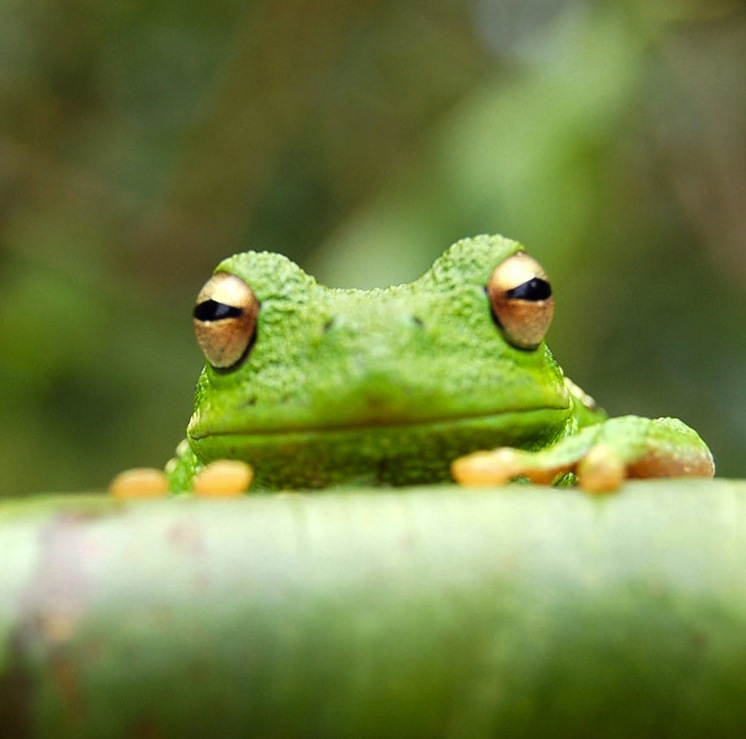
\includegraphics[width=0.3\textwidth]{frog.jpg}
\caption{\label{fig:frog}This frog was uploaded via the file-tree menu.}
\end{figure}

In the following, you can find the examples from the slides.

\begin{figure}[H]
    \centering
    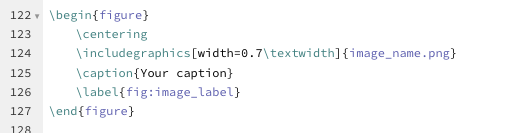
\includegraphics[width=0.7\textwidth]{figure_setup.png}
    \caption{The classic figure setup}
    \label{fig:fig_inception}
\end{figure}  

The classic \verb|\begin{figure}| consists of:\\
\vspace{1.5mm}
\begin{itemize}
    \item \verb|\includegraphics{}|: the name of the image you want to display
    \item \verb|\caption{}|: For captioning the image
    \item \verb|\label{}|: Label for cross-referencing
    \item \textit{caption} and \textit{label} are optional, but helpful
\end{itemize}

\subsubsection{Adjusting image size}

The picture below is scaled to cover 70\% of \textit{textwidth}.

\begin{figure}[H]
    \centering
    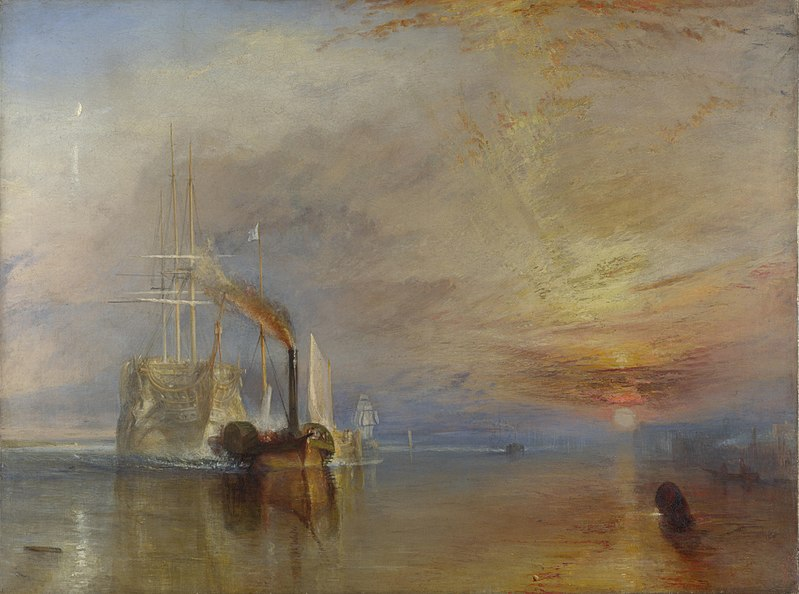
\includegraphics[width=0.7\textwidth]{temeraire.jpg}
    \caption{\textit{The Fighting Temeraire}, by JMW Turner (Source: \href{https://commons.wikimedia.org/wiki/File:The_Fighting_Temeraire,_JMW_Turner,_National_Gallery.jpg}{Wikimedia Commons})}
    \label{fig:temeraire_normal}
\end{figure} 

\newpage

Next, we'll scale the image to 10\% of its original size. The picture is rather big, so scaling it down to 10\% (scale=0.1) of its original size will look like this:

\begin{figure}[H]
    \centering
    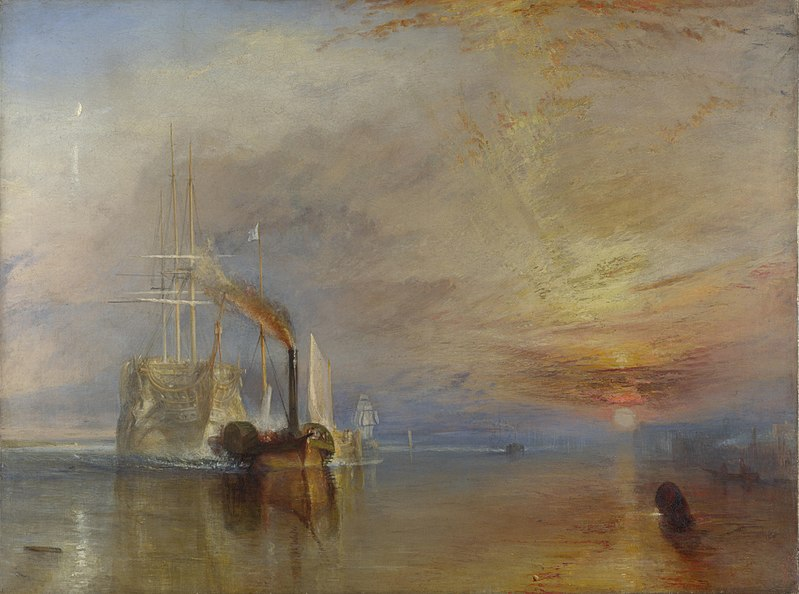
\includegraphics[scale=0.1]{temeraire.jpg}
    \caption{}
    \label{fig:temeraire_scale}
\end{figure} 

See \href{https://www.overleaf.com/learn/latex/Questions/How_do_I_specify_the_size_of_an_image_in_LaTeX\%3F}{here} for a short tutorial.

\subsubsection{Multiple images in one figure} Here's how to put multiple image into one figure. Specifically, you use the \textit{subfigure} environment.

\begin{figure}[H]
\begin{subfigure}{0.5\textwidth}
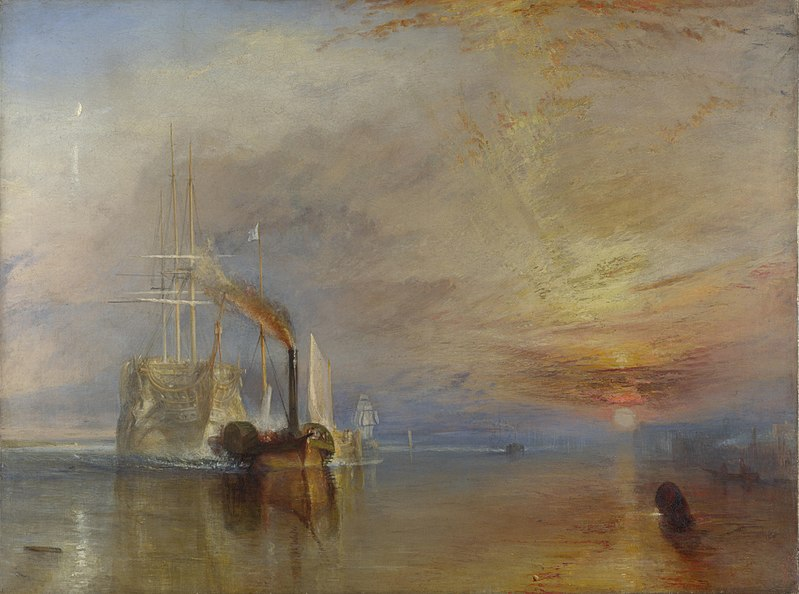
\includegraphics[width=0.9\linewidth, height=6cm]{temeraire.jpg} 
\caption{Caption 1}
\label{fig:subim1}
\end{subfigure}
\begin{subfigure}{0.5\textwidth}
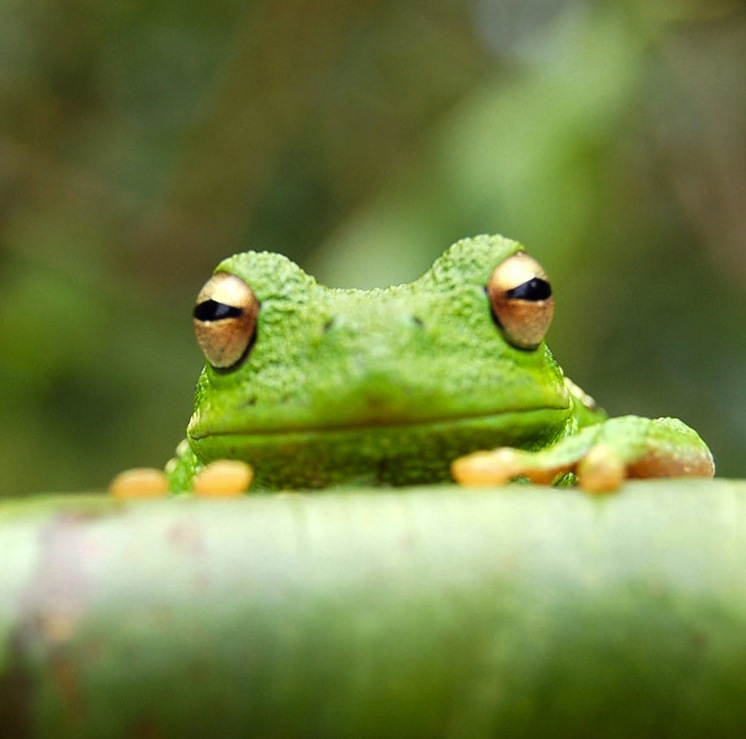
\includegraphics[width=0.9\linewidth, height=6cm]{frog.jpg}
\caption{Caption 2}
\label{fig:subim2}
\end{subfigure}
\caption{Caption for this figure with two images}
\label{fig:image2}
\end{figure}

This example is taken from the \href{https://www.overleaf.com/learn/latex/Positioning_images_and_tables\#Multiple_images_in_one_figure}{Overleaf tutorial}. You can label and thus reference the images separately. Figure \ref{fig:subim1} shows the painting by Turner, figure \ref{fig:subim2} shows a frog.

\subsection{How to add Tables}

Creating tables in LaTeX follows a specific formula, but there are many costumisation options.

\begin{figure}[H]
    \centering
    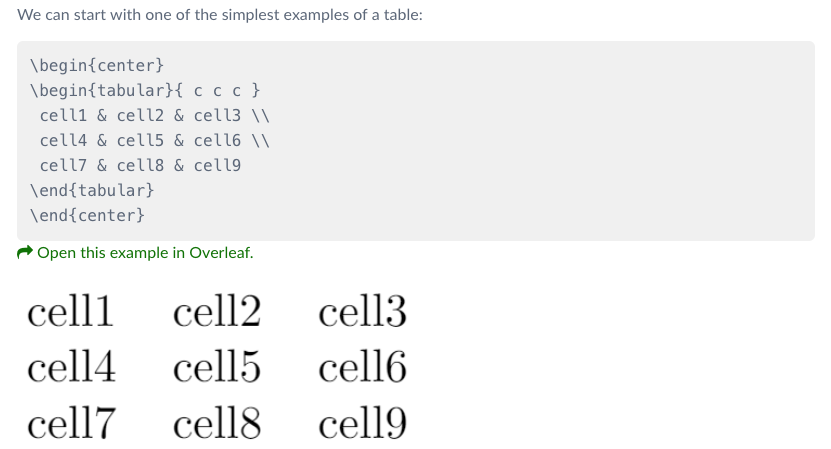
\includegraphics[width=0.8\textwidth]{table_simple.png}
    \caption{From the \href{https://www.overleaf.com/learn/latex/Tables}{Overleaf tutorial}}
    \label{fig:table_simple}
\end{figure}

\verb|\begin{tabular}{ c c c }| is the beginning of the tabular environment and \verb|{ c c c }| indicates that I am building a table with three columns.\\ 
The elements within each cell are to be \textbf{c}entered (\textbf{l} and \textbf{r} are also options).\\~\\
The elements of each row are separated by a \&, and you need to put \verb|\\| at the end to skip to the next row, if it exists.\\
You can add as many rows as you like.

If you want the columns separated by vertical lines, you can specify it by adding $\vert$ in between the c's:\\
\begin{figure}
    \centering
    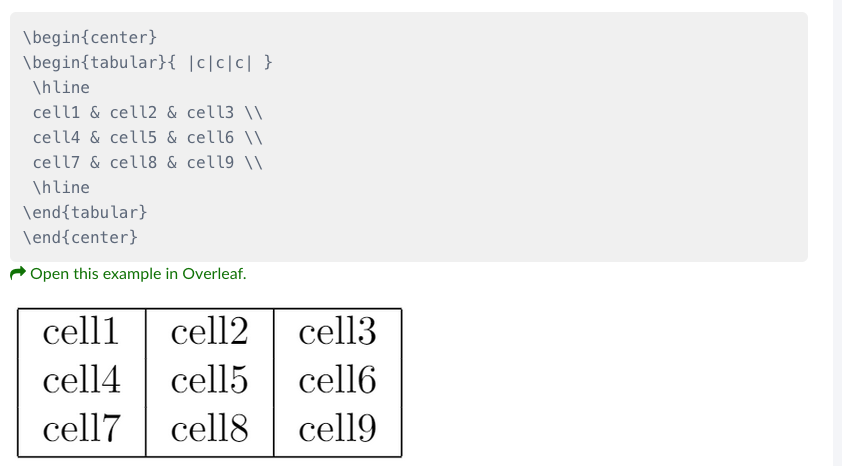
\includegraphics[width=0.75\textwidth]{tab_vert_bar.png}
    \caption{From the \href{https://www.overleaf.com/learn/latex/Tables}{Overleaf tutorial}}
    \label{fig:table_vertical}
\end{figure}

For horizontal lines, just insert \verb|\hline| in between rows. You can add as many of them as you want.\\
\begin{center}
\begin{tabular}{||c c c c||} 
 \hline
 Col1 & Col2 & Col2 & Col3 \\ [0.5ex] 
 \hline\hline
 1 & 6 & 87837 & 787 \\ 
 \hline
 2 & 7 & 78 & 5415 \\
 \hline
 3 & 545 & 778 & 7507 \\
 \hline
 4 & 545 & 18744 & 7560 \\
 \hline
 5 & 88 & 788 & 6344 \\ [1ex] 
 \hline
\end{tabular}
\end{center} 



Here, I make the top row a bit more spacious by inserting \verb|[0.5ex]| after the row as a whole. \textit{ex} is one of many ways to denote space in LaTeX, more common measures like cm, mm etc. work as well. You can find an overview below, taken from \href{https://tex.stackexchange.com/questions/8260/what-are-the-various-units-ex-em-in-pt-bp-dd-pc-expressed-in-mm}{StackOverflow}.

\begin{figure}[H]
    \centering
    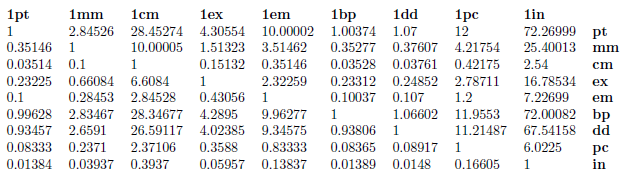
\includegraphics[width=0.8\textwidth]{spaces_latex.png}
    \label{fig:spaces}
\end{figure}

For quickly getting the basic syntax for a table, I recommend the \href{https://www.tablesgenerator.com/\#}{Table Generator}, see figure \ref{fig:table_generator} (or use ChatGPT).\\
\begin{figure}[H]
    \centering
    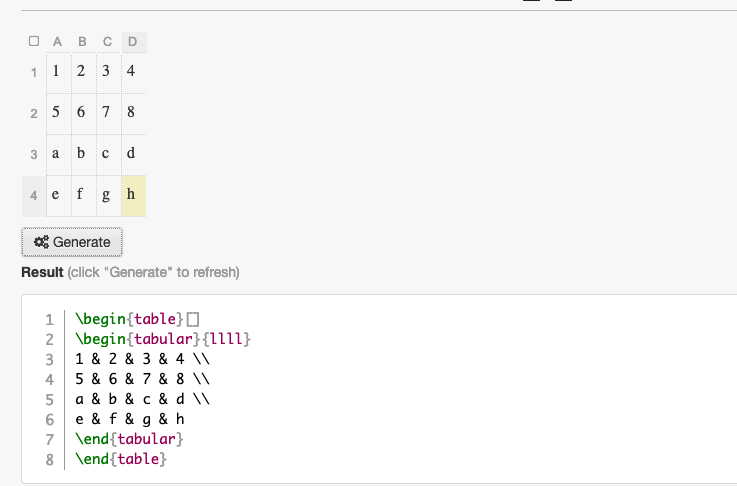
\includegraphics[width=0.6\textwidth]{table_generator.png}
    \caption{You can change and add to the template at will}
    \label{fig:table_generator}
\end{figure}

There is a range of parameters that will determine a table's (or figure's) placement. You wrap the \textit{tabular} environment into a more generic \textit{table} environment.\\
After \verb|\begin{table}|, put \verb|[h!]| (\textit{h} stands for \textit{here}) if you want to put the table exactly where it appears in the editor (i.e., exactly after one specific paragraph).\\
The ! overrides internal LaTeX parameters. Simply putting \verb|[h]| would merely put the table \textit{here, approximately}. 

\begin{itemize}
    \item \textbf{h} : place table or figure \textit{here}, approximately
    \item \textbf{t} : place table or figure at \textit{top} of the page
    \item \textbf{b} : place table or figure at \textit{bottom} of the page
    \item \textbf{p} : place table on special \textit{page}
    \item \textbf{!} : override internal LaTeX parameters
    \item \textbf{H} : roughly equal to h!
\end{itemize} 



\subsection{How to write Formulas}

\LaTeX{} is great at typesetting mathematics. Let $X_1, X_2, \ldots, X_n$ be a sequence of independent and identically distributed random variables with $\text{E}[X_i] = \mu$ and $\text{Var}[X_i] = \sigma^2 < \infty$, and let
\begin{equation*}
S_n = \frac{X_1 + X_2 + \cdots + X_n}{n}
      = \frac{1}{n}\sum_{i}^{n} X_i    
\end{equation*}

denote their mean. Then as $n$ approaches infinity, the random variables $\sqrt{n}(S_n - \mu)$ converge in distribution to a normal $\mathcal{N}(0, \sigma^2)$.\\

Examples from the slides:\\

Inline formulas and equations are written using \$ on each side.
E.g. $f(x) = x^2$ looks like this in an editor: \verb|$f(x) = x^2$|

Use two \$ at the beginning and need to center equations:
$$f(x) = x^2$$

Another option is to use the equation environment from the \textbf{amsmath} package.
This also adds numbers to equations by default.

\begin{equation}
    f(x) = x^2
\end{equation}  

\newpage

Fractions: $\frac{1}{x}$ is \verb|$\frac{1}{x}$|
\vspace{2mm}
\newline
\noindent Integral: $\int^a_b \frac{1}{3}x^3$ is \verb|$\int^a_b \frac{1}{3}x^3$|
\vspace{2mm}
\newline 
\noindent Sum: $\sum_{i=1}^n$ is \verb|$\sum_{i=1}^n$|\\~\\
You can use as many of these expressions in one equation as you need.\\

Use the \textit{align}-environment to align functions:\\
\begin{align*} 
2x - 5y &=  8 \\ 
3x + 9y &=  -12
\end{align*}

In order to align the expressions at the = sign, put an \& before it, like this: \verb|&=|

Some helpful resources for writing expressions:
\begin{itemize}
    \item \href{https://mirror.foobar.to/CTAN/macros/latex/required/amsmath/amsldoc.pdf}{User's guide}
    \item \href{https://en.wikibooks.org/wiki/LaTeX/Mathematics}{Wikibooks LaTeX/Mathematics} 
    \item \href{https://latex-tutorial.com/tutorials/amsmath/}{Intro} with common expressions
\end{itemize}
\vspace{2mm}
\subsubsection{Chemical expressions}
Photosynthesis: 6CO\textsubscript{2} + 6H\textsubscript{2}O $\rightarrow$ C\textsubscript{6}H\textsubscript{12}O\textsubscript{6} + 6O\textsubscript{2}

Chemical expressions and equations can be written using the \href{https://mirror.init7.net/ctan/macros/latex/contrib/mhchem/mhchem.pdf}{mhchem} package:\\ for example \ce{CO2 + C -> 2 CO} and \ce{Sb2O3}

\newpage

\section{How to add Citations and a References List}

You can simply upload a \verb|.bib| file containing your BibTeX entries, created with a tool such as JabRef. You can then cite entries from it, like this: \citet{dirac1981principles} (using \verb|citet{dirac1981principles}|) or this \citep{einstein1922general}. (using \verb|citep{einstein1922general}|. Cite several works by separating them with a comma.\\
\noindent Just remember to specify a bibliography style, as well as the filename of the \verb|.bib|. You can find a \href{https://www.overleaf.com/help/97-how-to-include-a-bibliography-using-bibtex}{video tutorial here} to learn more about BibTeX.\\
This example uses \textit{natbib}, a sort of add-on to the classic BibTeX setup. natbib is well suited for author-year style referencing. For other reference styles, BibTeX is usually enough.\\

More useful resources:
\begin{itemize}
    \item \href{https://de.overleaf.com/learn/latex/Bibliography_management_in_LaTeX}{Bibliography management in LaTeX}
    \item \href{https://www.overleaf.com/learn/latex/Bibtex_bibliography_styles}{BibTeX bibliography styles}
    \item \href{https://www.overleaf.com/learn/latex/Bibliography_management_with_natbib}{Bibliography management with natbib}
    \item \href{https://de.overleaf.com/learn/latex/Natbib_citation_styles}{natbib citation styles}
\end{itemize}   

\newpage
\bibliography{example}

\end{document}